\documentclass[12pt]{article}

\usepackage[T2A]{fontenc}
\usepackage[utf8]{inputenc}
\usepackage[english,russian]{babel}

\usepackage{amsmath,amsfonts,amssymb,amsthm,mathtools}

\usepackage[figurename=Рисунок]{caption}

\usepackage{graphicx} % Для вставки рисунков 
\graphicspath{{images/}{images2/}} % папки с картинками 
\DeclareGraphicsExtensions{.pdf,.png,.jpg}
\setlength\fboxsep{3pt} % Отступ рамки \fbox{} от рисунка 
\setlength\fboxrule{1pt} % Толщина линий рамки \fbox{} 
\usepackage{wrapfig} % Обтекание рисунков и таблиц текстом


\begin{document}
%начало титульного листа
\begin{titlepage}
\newpage
\begin{center}
\vspace{1cm}%расстояние до верхней строчки
\LARGE Московский Физико-Технический\\ Институт \\*
\vspace{5mm}
\large Факультет Биологической и Медицинской Физики\\*
\hrulefill %горизонтальная черта
\end{center}
\vspace{5em}
\begin{center}
\textbf{\huge Длинные линии} 
\end{center}
\vspace{20em}
\begin{flushright}
Выполнили: 
\hspace{1em}  
Яновская Дарья (6112)\\
Михайлова Анна (6112)\\
Колосов Семен (6112)\\
\vspace{1.5em}
\end{flushright}
\vspace{\fill}
\begin{center}
Москва 2019
\end{center}
\end{titlepage}
%конец титульного листа
 
\newpage

\begin{flushleft}
\section{ Цели работы}
%\vspace{1.5em}
\begin{itemize}
\item Ознакомиться с явлениями, связанными с передачей сигналов по длинным линиям и особенностями работы с линиями передачи сигналов.
\item Измерить характеристики коаксиального кабеля.
\item Исследовать стоячую волну в двухпроводной линии.
\item Получить наносекундные импульсы.
\item Собрать удвоитель напряжения.
\end{itemize}

\section{Теоретическая часть}
Во многих устройствах модули связаны между
собой с помощью линий передачи сигналов. Если длина лини  передачи сигнала больше длины электромагнитной волны, передаваемой по линии, в ней появляются эффекты, не
свойственные привычным электрическим цепям: волна может многократно отражаться от концов линии, искажаться
при распространении вдоль линии и так далее. Для описания данных явлений требуется рассматривать линию как среду, в которой распространяются электромагнитные волны.
\\
\vspace{1em}
Будем решать задачу о распространении гармонической электромагнитной волны вдоль линии передачи.
Пусть любые два размера линии много меньше длины волны, а третий – сравним или много больше. В таком случае исходная трехмерная задача сводится к одномерной задаче о распространении волны и двумерной задаче электро- и магнитостатики. Именно для такой ситуации и была разработана теория
длинных линий.

\subsection{Телеграфные уравнения}

Рассмотрим участок двухпроводной линии, длина которого $dx$ меньше длины волны $\lambda$.В таком случае для него выполняются правила Кирхгофа, используется модель с сосредоточенными параметрами. Также будем считать линию такой, что ее индуктивность, емкость, сопротивление, проводимость изоляции линейно увеличиваются с ростом длины рассматриваемого участка, в таком случае для описания линии можно ввести постоянные погонные параметры: $R_{x}, L_{x}, C_{x}, G_{x}$.

\begin{figure}[h]
\center{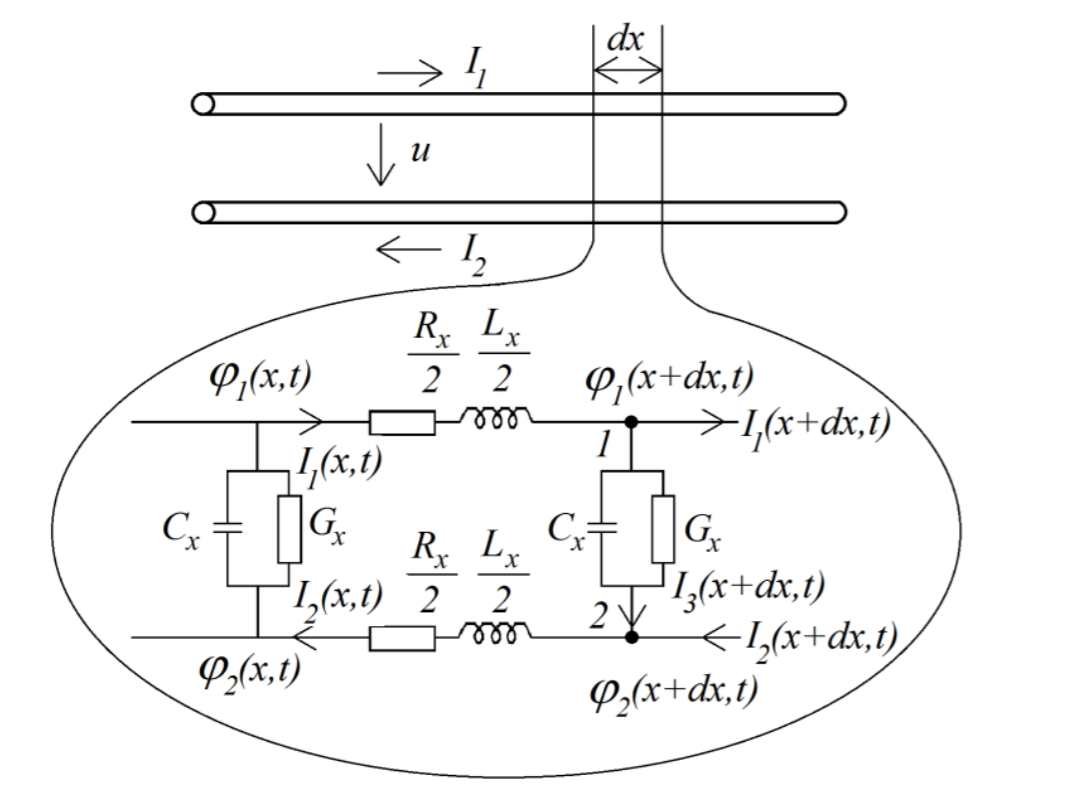
\includegraphics[width=10cm,height=7cm]{dl1}}
\caption{Эквивалентная электрическая схема участка линии.}
\label{ris:image}
\end{figure}

Система \textbf{телеграфных уравнений}:

\begin{equation}
\begin{cases}
-\frac{\partial I}{\partial x} = \left( G_{x} + C_{x} \frac{\partial}{\partial t} \right) u \\
-\frac{\partial u}{\partial x} = \left( R_{x} + L_{x} \frac{\partial}{\partial t} \right) I
 \end{cases}
\end{equation}
Преобразуя систему, получим уравнение:
\begin{equation}
\frac{\partial^2 A(x, \omega)}{\partial x^2} - \left[ \gamma(\omega)\right]^2 A(x, \omega)= 0
\end{equation}
Решение такого уравнения известно:
\begin{equation}
A(x, \omega) = C_{1}sh[\gamma(\omega)x]+ C_{2}ch[\gamma(x)x]
\end{equation}
\subsection{Распространение электромагнитной волны вдоль линии}
Перепишем (2) в виде:
\begin{equation}
A(x,\omega)=\frac{C_2 - C_1}{2}e^{-\gamma(\omega)x} + \frac{C_2 + C_1}{2}e^{\gamma(\omega)x} = A_1e^{-\gamma(\omega)x} + A_2e^{\gamma(\omega)x}
\end{equation}

Ввели обозначение
\begin{equation}
\gamma(\omega)=\alpha(\omega)+i\beta(\omega)
\end{equation}
где $\alpha$ - \textbf{затухание на частоте f}, $f=\frac{\omega}{2\pi}$, показывает, насколько  изменяется амплитуда синусоидальной волны при распространении вдоль линии,\\
$\beta$ - \textbf{фазовая постоянная на частоте f}, отражает изменение фазы волны при распространении вдоль линии, $\lambda = \frac{2\pi}{\beta}$\\
\vspace{1em}
Каждая компонента сложной волны, распространяющейся по линии, является суммой двух бегущих волн. Первое слагаемое
(4) отвечает волне, распространяющейся в направлении оси абсцисс(\textbf{падающая волна} - распространяется от генератора), второе – волне, распространяющейся против направления оси (\textbf{отраженная}).  Падающая волна при удалении от генератора экспоненциально затухает.\\
Комплексная амплитуда тока:
\begin{equation}
B(x,\omega) = \frac{A_1e^{-\gamma(\omega)x} - A_2e^{\gamma(\omega)x}}{\Omega(\omega)}
\end{equation}
где
\begin{equation}
\Omega(\omega)=\frac{R_x + i\omega L_x}{\gamma(\omega)}=\sqrt{\frac{R_x + i\omega L_x}{G_x + i\omega C_x}}
\end{equation}
$\Omega$ - \textbf{волновое сопротивление или характеристический импеданс}\\
Физический смысл: отношение комплексных амплитуд
напряжения между проводами линии и тока в линии для синусоидальной компоненты сложной электромагнитной волны, соответствующей частоте $\omega$.
\subsection{Отражения волн в линиях передачи}
В заданной точке линии в заданный момент времени напряжение описывается соотношением
\begin{equation}
u(x,t) =\left( A_1e^{-\gamma(\omega)x} + A_2e^{\gamma(\omega)x}\right)e^{i\omega t}
\end{equation}
Отраженная волна
появляется в той точке, где линия соединяется с нагрузкой (в появлении отраженной волны «виновата» нагрузка).
Обозначим
\begin{equation}
u_{\text{пад}}(x,t) = A_1e^{-\gamma(\omega)x}e^{i\omega t}
\hspace{1cm}
u_{\text{отр}}(x,t) = A_2e^{\gamma(\omega)x}e^{i\omega t}
\end{equation}
Таким образом возникает \textbf{коэффициент отражения по напряжению}
\begin{equation}
r_u(\omega)=\frac{u_{\text{отр}}(l,t)}{u_{\text{пад}}(l,t)} = \frac{ Z_H(\omega) -\Omega(\omega)}{Z_H(\omega) +\Omega(\omega)}
\end{equation}
Rоэффициент отражения не зависит от длины линии, затухания или времени и определяется только волновым сопро
тивлением линии и импедансом нагрузки. В общем случае коэффициент
отражения – комплексное число, зависящее от частоты.\\
Напряжение (или ток) в заданной точке линии является результатом сложения всех компонент, включая отраженные. \\
Генератор, обладая определенным собственным импедансом, также является источником отраженных волн. В качестве источников отражений, помимо концов линии, также выступают дефекты линии. 
\subsection{Режимы работы линии, формирование стоячих волн в линии}
\begin{enumerate}
\item \textbf{Режим короткого замыкания:} в
качестве нагрузки к линии подключен шунт с нулевым сопротивлением
(или в нагрузке произошло короткое замыкание, или два провода линии
просто соединили, и никакой нагрузки нет). $Z_H=0$ и $r_u =-1$. Энергия в нагрузку не передается и полностью
рассеивается в линии и на внутреннем сопротивлении генератора.
\item \textbf{Режим холостого хода:} к линии ничего не подключено, то есть ток через
«нагрузку» равен нулю. $Z_H \rightarrow \infty$ и $r_u = 1$. Энергия в нагрузку не передается и полностью рассеивается в линии и на внутреннем сопротивлении генератора. 
\item \textbf{Режим согласованной работы:} импеданс нагрузки в точности равен волновому сопротивлению линии. $Z_H= \Omega$ и $r_u =0$.Отраженная волна отсутствует. Энергия практически
полностью передается от генератора в нагрузку, лишь немного рассеиваясь в линии. 
\end{enumerate}
\begin{figure}[!h]
\center{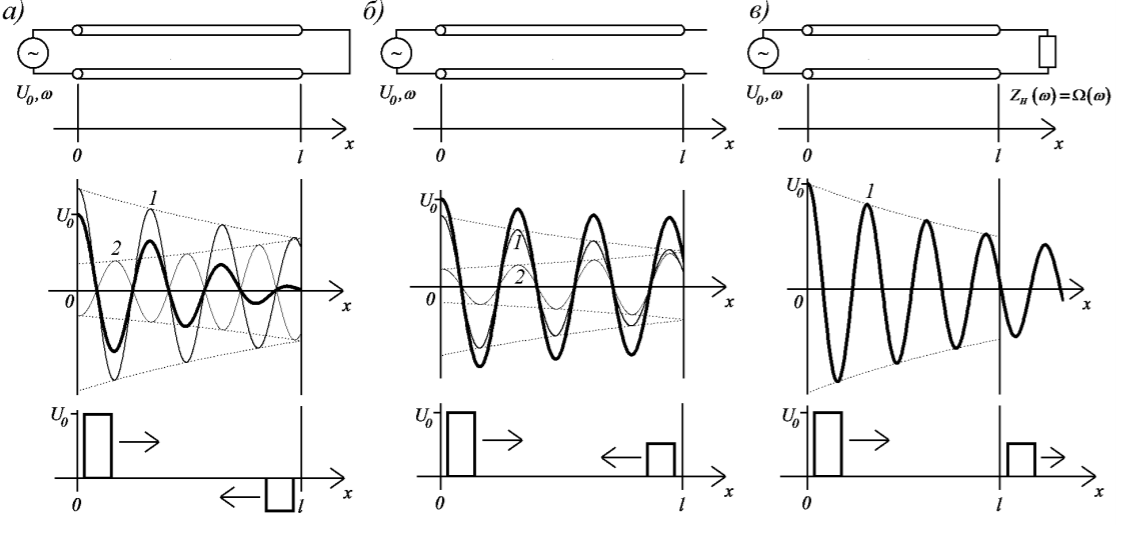
\includegraphics[width=16cm,height=7cm]{dl2}}
\caption{Режимы работы линии: а) короткое замыкание б) холостой ход в) согласованная работа. 1 - падающая, 2 - отраженная.}
\label{ris:image}
\end{figure}
Уравнение \textbf{стоячей волны}:
\begin{equation}
u(x,t) = U_0 \sin (\omega t - \beta x) + U_0 \sin (\omega t + \beta x)=2U_0 \cos (\beta x)\sin (\omega t)
\end{equation}
Для описания точности согласования часто используют
коэффициент бегущей волны (КБВ) и коэффициент стоячей волны
(КСВ), КСВ = 1/КБВ.\\
КСВН есть отношение минимума амплитуды колебаний напряжения в смешанной волне к максимуму КСВН = $|U|_{min}/|U|_{max}$.\\
При отсутствии затухания:
\begin{equation}
\text{КСВН} = \frac{|U|_{\text{пад}}-|U|_{\text{отр}}}{|U|_{\text{пад}}+|U|_{\text{отр}}} = \frac{1-|r_u|}{1+|r_u|}
\end{equation}
\subsection{Фазовая и групповая скорости. Понятие о сигнале}
Сигнал – материальный носитель информации, используемый для
передачи сообщений из одного пункта в другой. Сигналом может
быть любой физический процесс, параметры которого изменяются в
соответствии с передаваемым сообщением.\\
Информация, содержащаяся в сообщении и передаваемая с помощью сигнала, представляется
изменением одного или нескольких параметров сигнала – его амплитуды (интенсивности), длительности, частоты, ширины спектра, фазы, времени запаздывания, поляризации и т.п. Соответственно, сигнал должен обладать параметрами, которые можно измерять и которые изменяются в зависимости от содержания сообщения.\\
\vspace{0.5cm}
С помощью синусоидальных токов также невозможно передавать сообщения, так как все параметры синусоиды с течением времени не
изменяются.
Любые изменения синусоидальных колебаний напряжения (или тока), будь то изменение амплитуды, частоты или скачок фазы, приводят к появлению в
спектре частот, отличных от исходной частоты колебаний.
Говорить о сигнале
можно только в том случае, если спектр колебаний измеряемого параметра содержит более одной частоты.\\
С \textbf{фазовой скоростью} перемещается точка постоянной фазы гармонической волны:
\begin{equation}
V_{\text{ф}} = \lim_{\Delta t\to0}\frac{\Delta x}{\Delta t} = \frac{\omega}{\beta (\omega)}
\end{equation}
\textbf{Групповая скорость} описывает перемещение группы гармонических волн как единого целого:
\begin{equation}
V_{\text{гр}} = \lim_{\Delta t\to0}\frac{\Delta x}{\Delta t} = \frac{\Delta \omega}{\Delta \beta}
\end{equation}
Групповая скорость (в отличие от фазовой) является скоростью передачи информации или энергии электромагнитного поля и потому, согласно постулату Эйнштейна, не может превосходить скорость света в вакууме.\\
\textbf{Формула Рэлея:}
\begin{equation}
V_{\text{гр}} = V_{\text{ф}} - \lambda \frac{dV_{\text{ф}}}{d\lambda}
\end{equation}
\subsection{Частотная характеристика линии}
Рассмотрим прием исследования, при котором, действуя на объект, регистрируют его реакцию и находят связи между воздействием и откликом
объекта.\\
Для описания линейных пассивных объектов можно использовать частотную характеристику. Линейность - ответ на гармоническое воздействие гармонический, частоты реакции и воздействия совпадают для любой частоты. Пассивность - нет воздействия $\Rightarrow$ нет отклика.\\
\vspace{0.5cm}
Модуль частотной характеристики - отношениt
амплитуды отклика к амплитуде воздействия \textbf{(АЧХ)}. Аргумент частотной характеристики равен разности фаз отклика и воздействия \textbf{(ФЧХ)}.\\
Рассмотрим задачу о нахождении напряжения в заданный момент времени в
заданной точке нагруженной линии.\\
Частотная характеристика:
\begin{equation}
f(\omega ,x) = \frac{f(x,\omega)}{f(0,\omega)} = e^{-\gamma (\omega)x} \frac{1+r_u(\omega)e^{-2\gamma (\omega )(l-x)}}{1+r_u(\omega )e^{-2\gamma (\omega )l}}
\end{equation}
Если нагрузка согласована(отражений нет), то частотная характеристика для величины напряжения на нагрузке равной величине напряжения на правом конце нагруженной линии:
\begin{equation}
f(\omega ,x) = e^{-\gamma (\omega)l} 
\end{equation}
\begin{equation}
\begin{cases}
\alpha^2 (\omega ) - \beta^2 (\omega ) = R_xG_x - \omega^2 L_xC_x \\
2\alpha (\omega )\beta (\omega ) = \omega (L_xG_x - R_xC_x)
 \end{cases}
\end{equation}
Построив графики в осях
\begin{equation}
Y_1 = \alpha^2 (\omega ) - \beta^2 (\omega ) ,\hspace{1cm} X_1 = \omega^2 
\end{equation}
\begin{equation}
Y_2 = 2\alpha (\omega )\beta (\omega ) ,\hspace{1.5cm} X_2 = \omega
\end{equation}
если $R_x, G_x, L_x, C_x$ не зависят от частоты, получим две прямые. Из коэффициентов наклона прямых $y = ax + b$ находим: $a_1 = -L_xC_x, b_1 = R_xG_x,
a_2 = (L_xG_x + R_xC_x), b_2 = 0$.
В случае линии с малыми потерями $R_x\ll\omega L_x, G_x \approx 0$ получаем
\begin{equation}
a_1 = -L_xC_x,\hspace{0.5cm} b_1 \approx 0, \hspace{0.5cm} a_2 =  R_xC_x,\hspace{0.5cm} \Omega \approx \sqrt{\frac{l_x}{C_x}}
\end{equation}
\newpage
\subsection{Кабельные формирователи импульсов и трансформаторы}
\begin{figure}[!h]
\center{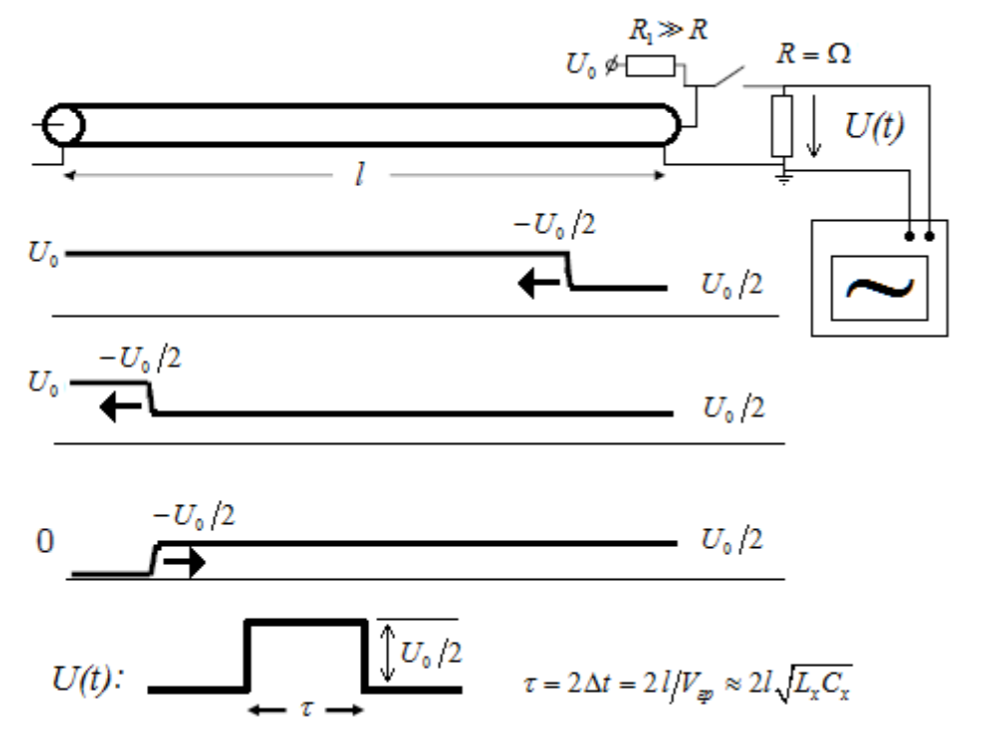
\includegraphics[width=16cm,height=13cm]{dl3}}
\caption{Одинарная формирующая линия.}
\label{ris:image}
\end{figure}
\section{Экспериментальная часть}
\subsection{Согласование линии, коэффициент отражения}
В работе в качестве линии передачи используется коаксиальный кабель длиной l=31 м. Получили отраженный импульс для режимов холостого хода и короткого замыкания. Подключив к линии резистор переменного сопротивления, согласуем линию с нагрузкой, определив тем самым \textbf{волновое сопротивление линии $\Omega =87,1$ Ом}.

\begin{figure}[!h]
\center{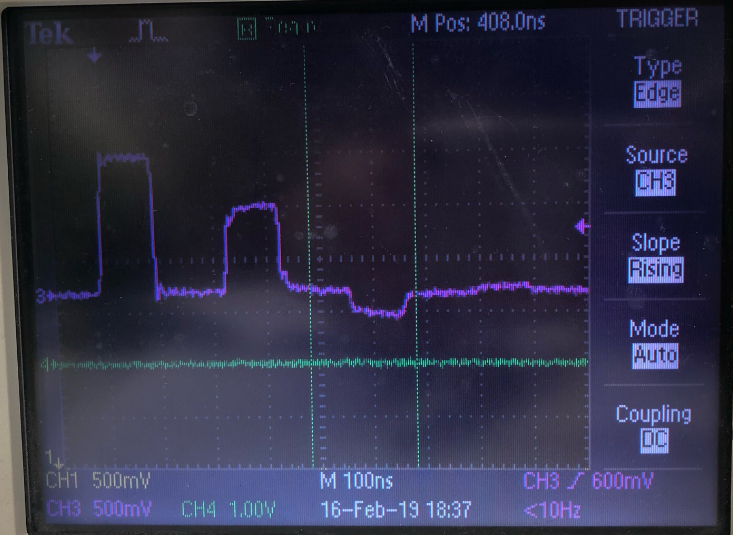
\includegraphics[width=16cm,height=13cm]{dl4}}
\caption{Работа в режиме холостого хода.}
\label{ris:image}
\end{figure}
\begin{table}[!h]
\caption{Характеристики осциллограммы (амплитуды импульсов и временные промежутки между их передними фронтами) и коэффициенты отражения для режимов короткого замыкания и холостого хода.}
\begin{tabular}{lllll}
                           & \text{Холостой ход} & \text{Короткое замыкание} & r\text{(х.х.)} & r\text{(к.з.)} \\
$\Delta V_1$ & 1.31         & 1.31               & 0.641   & 0.605   \\
$\Delta V_2$                  & 0.84         & 0.792              & 0.238   & 0.273   \\
$\Delta V_3$                  & 0.2          & 0.216              & 0.280   & 0.296   \\
$\Delta V_4$                  & 0.056        & 0.064              &         &         \\
$\Delta t$                   & 0.104        & 0.108              &         &        
\end{tabular}
\end{table}

\subsection{Измерение АЧХ и ФЧХ коаксиального кабеля}
При работе в режиме согласованной нагрузки подали в линию непрерывное синусоидальное напряжение, измерили отношение амплитуд напряжения, подаваемого в линию и регистрируемого на нагрузке, и разность фаз между ними для области частот 100 кГц – 50 МГц.

\begin{figure}[!h]
\center{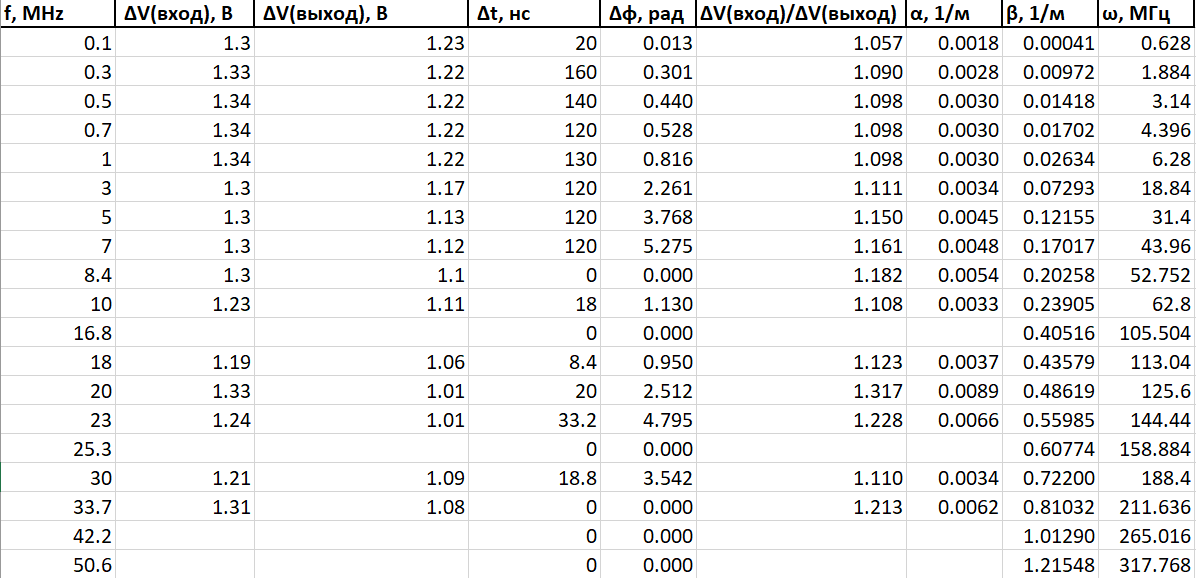
\includegraphics[width=16cm,height=8cm]{dl14}}
\caption{Исследование АЧХ и ФЧХ.}
\label{ris:image}
\end{figure}
\subsubsection{Для коаксиального кабеля по измеренным АЧХ и ФЧХ построим $\alpha (\omega)$ и $\beta (\omega)$}
\begin{figure}[!h]
\center{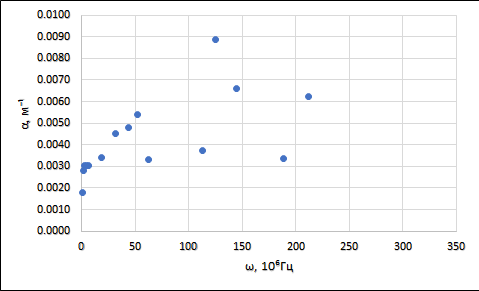
\includegraphics[width=12cm,height=7cm]{dl15}}
\caption{АЧХ (амплитудно-частотная характеристика.}
\label{ris:image}
\end{figure}
\begin{figure}[!h]
\center{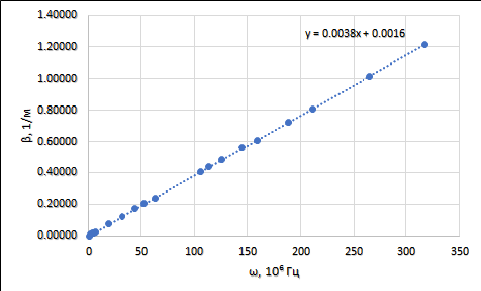
\includegraphics[width=12cm,height=7cm]{dl16}}
\caption{ФЧХ ( фазо-частотная характеристика.}
\label{ris:image}
\end{figure}
\subsubsection{Построим линеаризованные зависимости}
\begin{figure}[!h]
\center{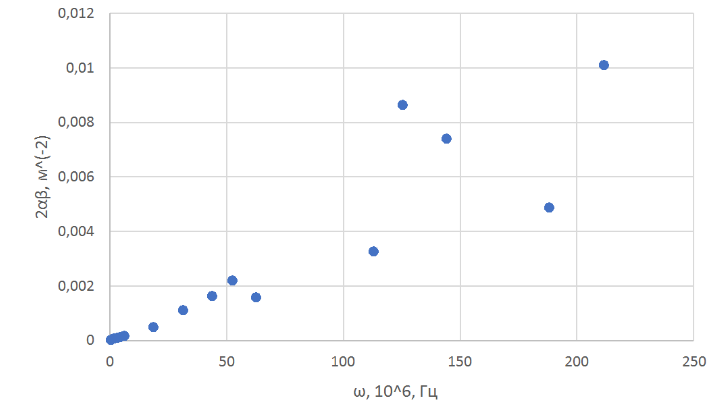
\includegraphics[width=12cm,height=7cm]{dl22}}
\caption{Линеаризованная зависимость Y2 (X2).}
\label{ris:image}
\end{figure}
\begin{figure}[!h]
\center{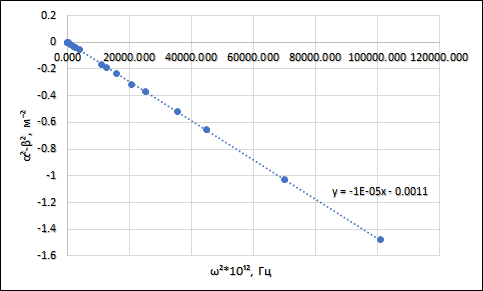
\includegraphics[width=12cm,height=7cm]{dl18}}
\caption{Линеаризованная зависимость Y1(X1).}
\label{ris:image}
\end{figure}
Рассчитаем погонные параметры по формулам :
\begin{equation}
\left[
  \begin{array}{ccc}
     C_x = \sqrt{-\frac{a_1}{\Omega}} \\
     L_x = \Omega\sqrt{-a_1} \\
     R_x = \frac{a_2}{C_x} \\
  \end{array}
\right.
\end{equation}
$L_x = 0.27 \pm 0.1 \frac{\text{мкГН}}{\text{м}}$ \hspace{1cm} $C_x = 34 \pm 2 \frac{\text{пФ}}{\text{м}}$
\subsubsection{Построим зависимость $R_x(\omega)$.}

\begin{table}[!h]
\caption{Зависимость погонного напряжения от частоты генератора.}
\begin{tabular}{lll}
$\omega$, МГц  & $\omega ^{1/2}$, МГц$^{1/2}$ & $R_x$, Ом/м \\
16,014  & 4,002                                            & 0,83     \\
22,922  & 4,788                                            & 1,1      \\
27,946  & 5,286                                            & 1,1      \\
137,218 & 11,714                                           & 1,3      \\
137,218 & 11,714                                           & 1,6     
\end{tabular}
\end{table}
\begin{figure}[!h]
\center{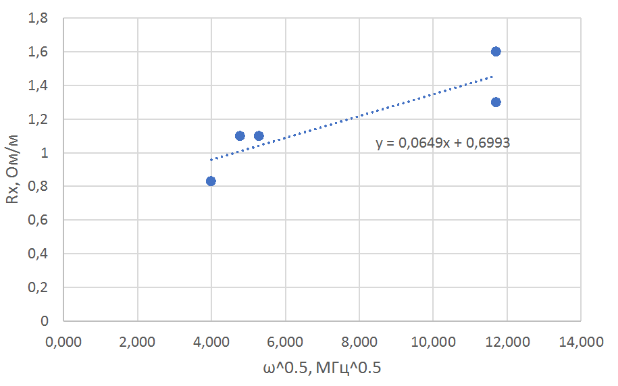
\includegraphics[width=12cm,height=7cm]{dl19}}
\caption{Зависимость погонного сопротивления от частоты генератора.}
\label{ris:image}
\end{figure}
Нелинейность графика 8 обусловлена скин-эффектом.

Построили кусочно-линейную аппроксимацию графика, каждый линейный фрагмент должен описывать 5–7 точек. Для построения графика использовали значения частот, соответствующих серединам линейных фрагментов.
\subsubsection{Построим зависимость фазовой скорости от частоты}
\begin{figure}[!h]
\center{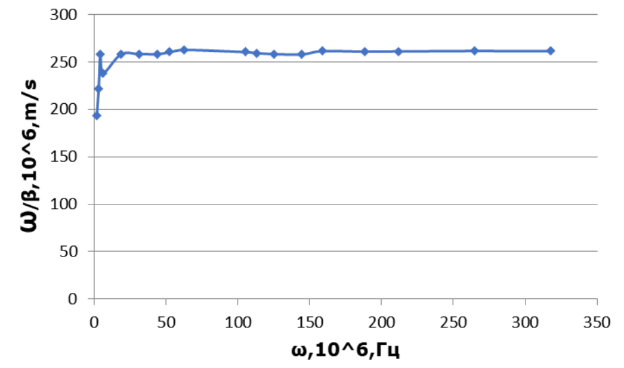
\includegraphics[width=12cm,height=7cm]{dl20}}
\caption{Зависимость фазовой скорости от частоты.}
\label{ris:image}
\end{figure}
Рассчитанная групповая скорость $V_{\text{гр}}= \frac{1}{\partial \beta / \partial \omega} = (2.63 \pm 0.04) 10^8$ м/c.
\subsection{Кабельный трансформатор, формирователь импульса}
\subsubsection{Формирователь импульса}
Зная групповую скорость для коаксиального кабеля, рассчитаем зависимость ожидаемой длительности импульса от длины линии для формирователя импульса по формуле $\tau = 2\Delta t = \frac{2l}{V_{\text{гр}}} \approx 2l\sqrt{C_xL_x}$.
\begin{table}[!h]
\caption{Зависимость длительности импульса от длины линии.}
\begin{tabular}{lllll}
l, м & $\tau$, нс & $2l\sqrt{C_xL_x} $, нс & $\frac{2l}{V_{\text{гр}}}$, нс & $\tau$, нс погр \\
31  & 236  & 196.0319996       & 221.4286  & 3.3     \\
7   & 53   & 44.26529024       & 50        & 0.71    \\
14  & 108  & 88.53058048       & 100       & 1.44   
\end{tabular}
\end{table}
\begin{figure}[!h]
\center{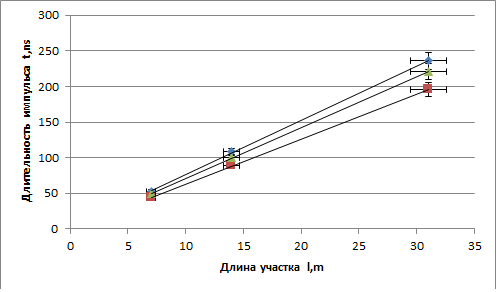
\includegraphics[width=12cm,height=7cm]{dl21}}
\caption{Зависимость длительности импульса от длины волны.}
\label{ris:image}
\end{figure}
\newpage
\subsubsection{Трансформатор}
Для умножителя напряжений рассчитаем коэффициент умножения $r_u = \frac{U_{\text{пад}}}{U_{\text{отр}}} = \frac{U_{\text{нагр}}}{U_{\text{ген}}}$ для длительностей импульса $\tau_1 = 100$нс и $\tau_1 = 10000$ нс.

Получается, что коэффициент умножения зависит от длительности импульса.
\begin{table}[!h]
\caption{Исследование трансформации сигнала.}
\begin{tabular}{llll}
$Vg,mV$ & $Vn,mV$ & $\tau,ns$  & $r_u$  \\
491   & 889   & 100   & 1.81 \\
569   & 990   & 10000 & 1.74
\end{tabular}
\end{table}
\subsubsection{Сигналы, полученные на осциллографе при формировании импульсов}
\begin{figure}[!h]
\center{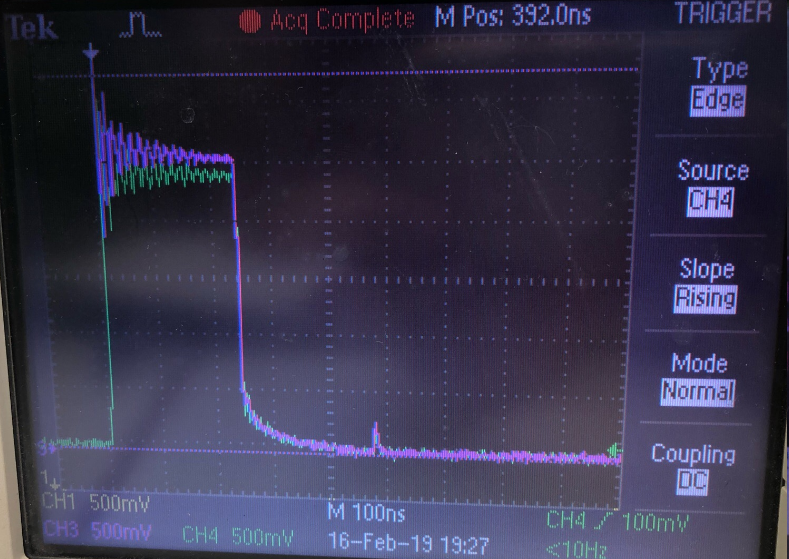
\includegraphics[width=10cm,height=6cm]{dl6}}
\caption{Формирование импульса при длине коаксиального кабеля $l=31$м.}
\label{ris:image}
\end{figure}
\begin{figure}[!h]
\center{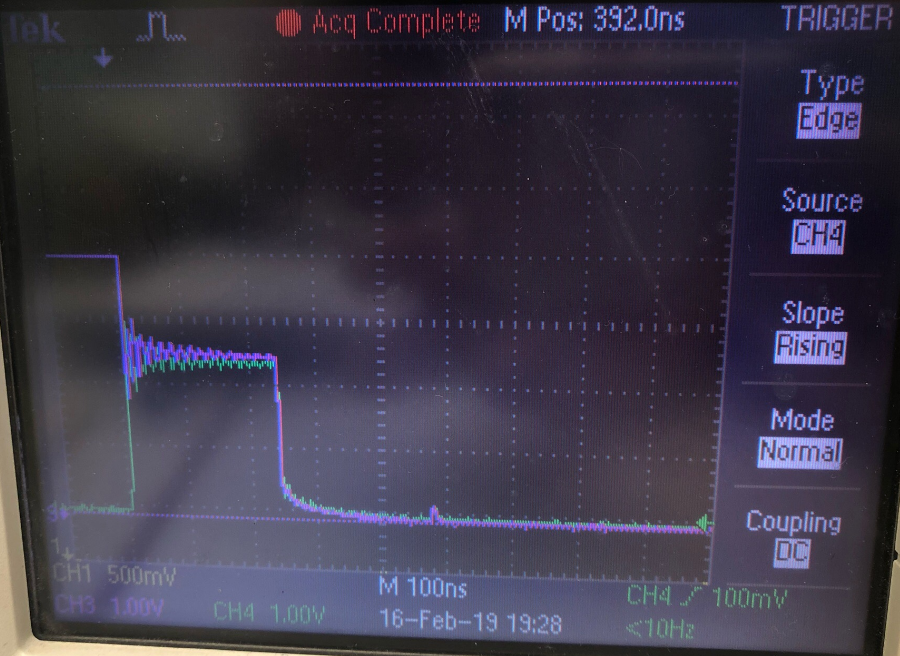
\includegraphics[width=10cm,height=6cm]{dl7}}
\caption{Формирование импульса при длине коаксиального кабеля $l=7$м.}
\label{ris:image}
\end{figure}
\begin{figure}[!h]
\center{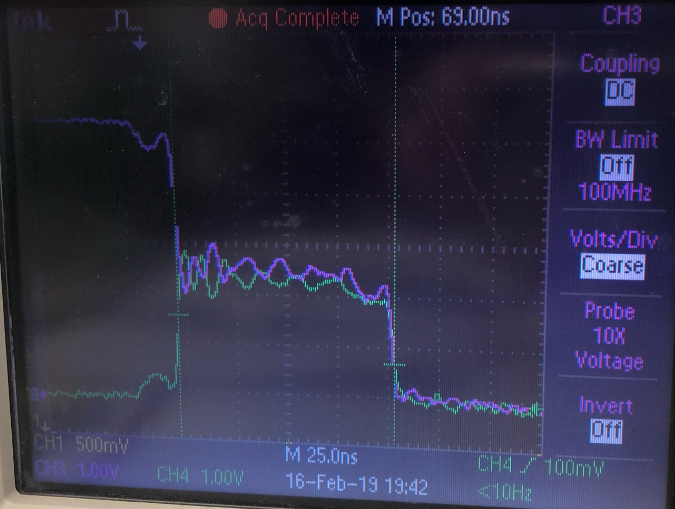
\includegraphics[width=10cm,height=6cm]{dl8}}
\caption{Формирование импульса при длине коаксиального кабеля $l=14$м.}
\label{ris:image}
\end{figure}
\subsubsection{Сигналы, полученные на осциллографе при работе в режиме трансформатора}
\begin{figure}[!h]
\center{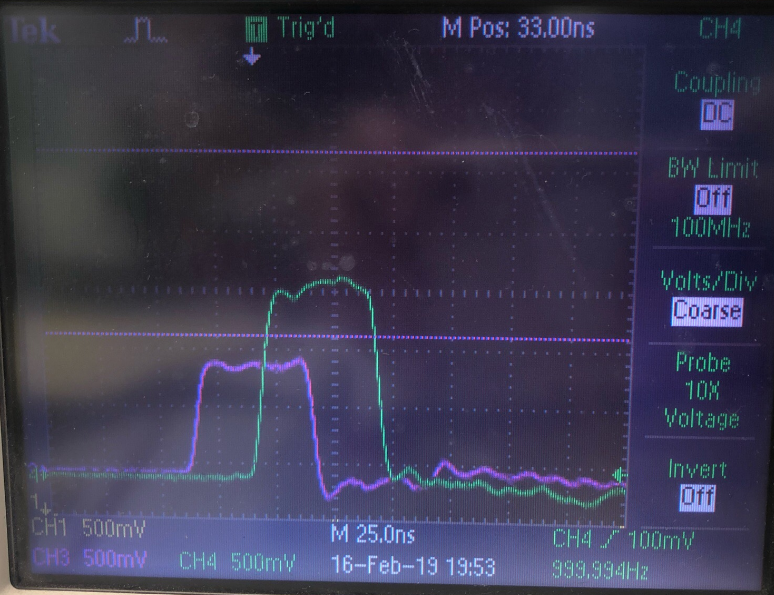
\includegraphics[width=10cm,height=6cm]{dl10}}
\caption{Трансформация сигнала при длине импульса$100$нс.}
\label{ris:image}
\end{figure}
\begin{figure}[!h]
\center{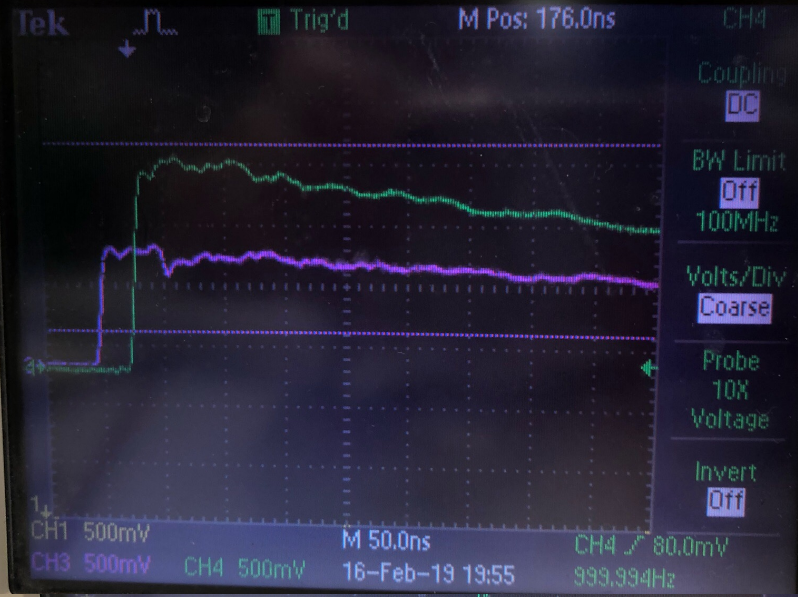
\includegraphics[width=10cm,height=6cm]{dl12}}
\caption{Трансформация сигнала при длине импульса$10000$нс.}
\label{ris:image}
\end{figure}
\newpage
Для коаксиального кабеля, исходя из найденной величины погонной емкости, рассчитаем относительную диэлектрическую проницаемость материала изоляции (в системе Си для коаксиального кабеля $C_x = \frac{2\pi \epsilon \epsilon_0}{\ln(D/d)}$ D – внутренний диаметр экрана (5 мм), d – диаметр центральной жилы (1 мм)). Материал изоляции коаксиального кабеля – вспененный воздухом полиэтилен, оцените объемную долю воздуха в изоляции, если для чистого полиэтилена $\epsilon = 2.25$.
\[
\epsilon = 1.13 \pm 0.03 
\]
\[\epsilon = \alpha \epsilon_{\text{возд}} + (1-\alpha) \epsilon_{\text{полиэт}} \]
\[\alpha = 0.9 \pm 0.02\]
\section{Вывод}
В результате выполнения работы были измерены и получены:
\begin{itemize}
\item АЧХ и ФЧХ коаксиального кабеля
\item Зависимости $\alpha (\omega)$ и $\beta (\omega)$.
\item Рассчитаны погонные параметры линии, фазовая скорость: $L_x = 0.27 \pm 0.1 \frac{\text{мкГН}}{\text{м}}$ \hspace{0.5cm} $C_x = 34 \pm 2 \frac{\text{пФ}}{\text{м}}$ \hspace{0.5cm} $V_{\text{гр}}= (2.63 \pm 0.04) 10^8$ м/c.
\item Для коаксиального кабеля, исходя из найденных погонных параметров, рассчитана относительная диэлектрическая проницаемость материала изоляции, оценена объемная доля в изоляции: $\epsilon = 1.13 \pm 0.03$, $\alpha = 0.9 \pm 0.02$
\item Для умножителя напряжения рассчитали коэффициент умножения для различных длительностей импульса. Был сделан вывод, что коэффициент умножения зависит от длительности импульса. Импульс продолжительностью 10000нс сильно исказился из-за того, что для него линия уже не была длинной.
\end{itemize}
\section{Список литературы}
1. «Длинные линии». Учебно-методическое пособие / Сост. Ю. С. Семенов. – М.: МФТИ, 2015. – 51 с.

2. «Физические методы исследования. 2. Сигналы в длинных линиях»: Учебно-методическое пособие / Сост.: А. В. Максимычев. – М.: МФТИ, 2007. - 44 с.
\end{flushleft}
\end{document}